% ch07: 原文 GLDraft_D.tex 行 1383–1765；§4.3
% 只译散文（标题、正文、图题、脚注）；公式、\label、\ref、\eqref、\cite、图文件名保持不变。

\subsection{对偶 't Hooft 算符}\label{dualhooft}

 \begin{figure}
 \begin{center}
   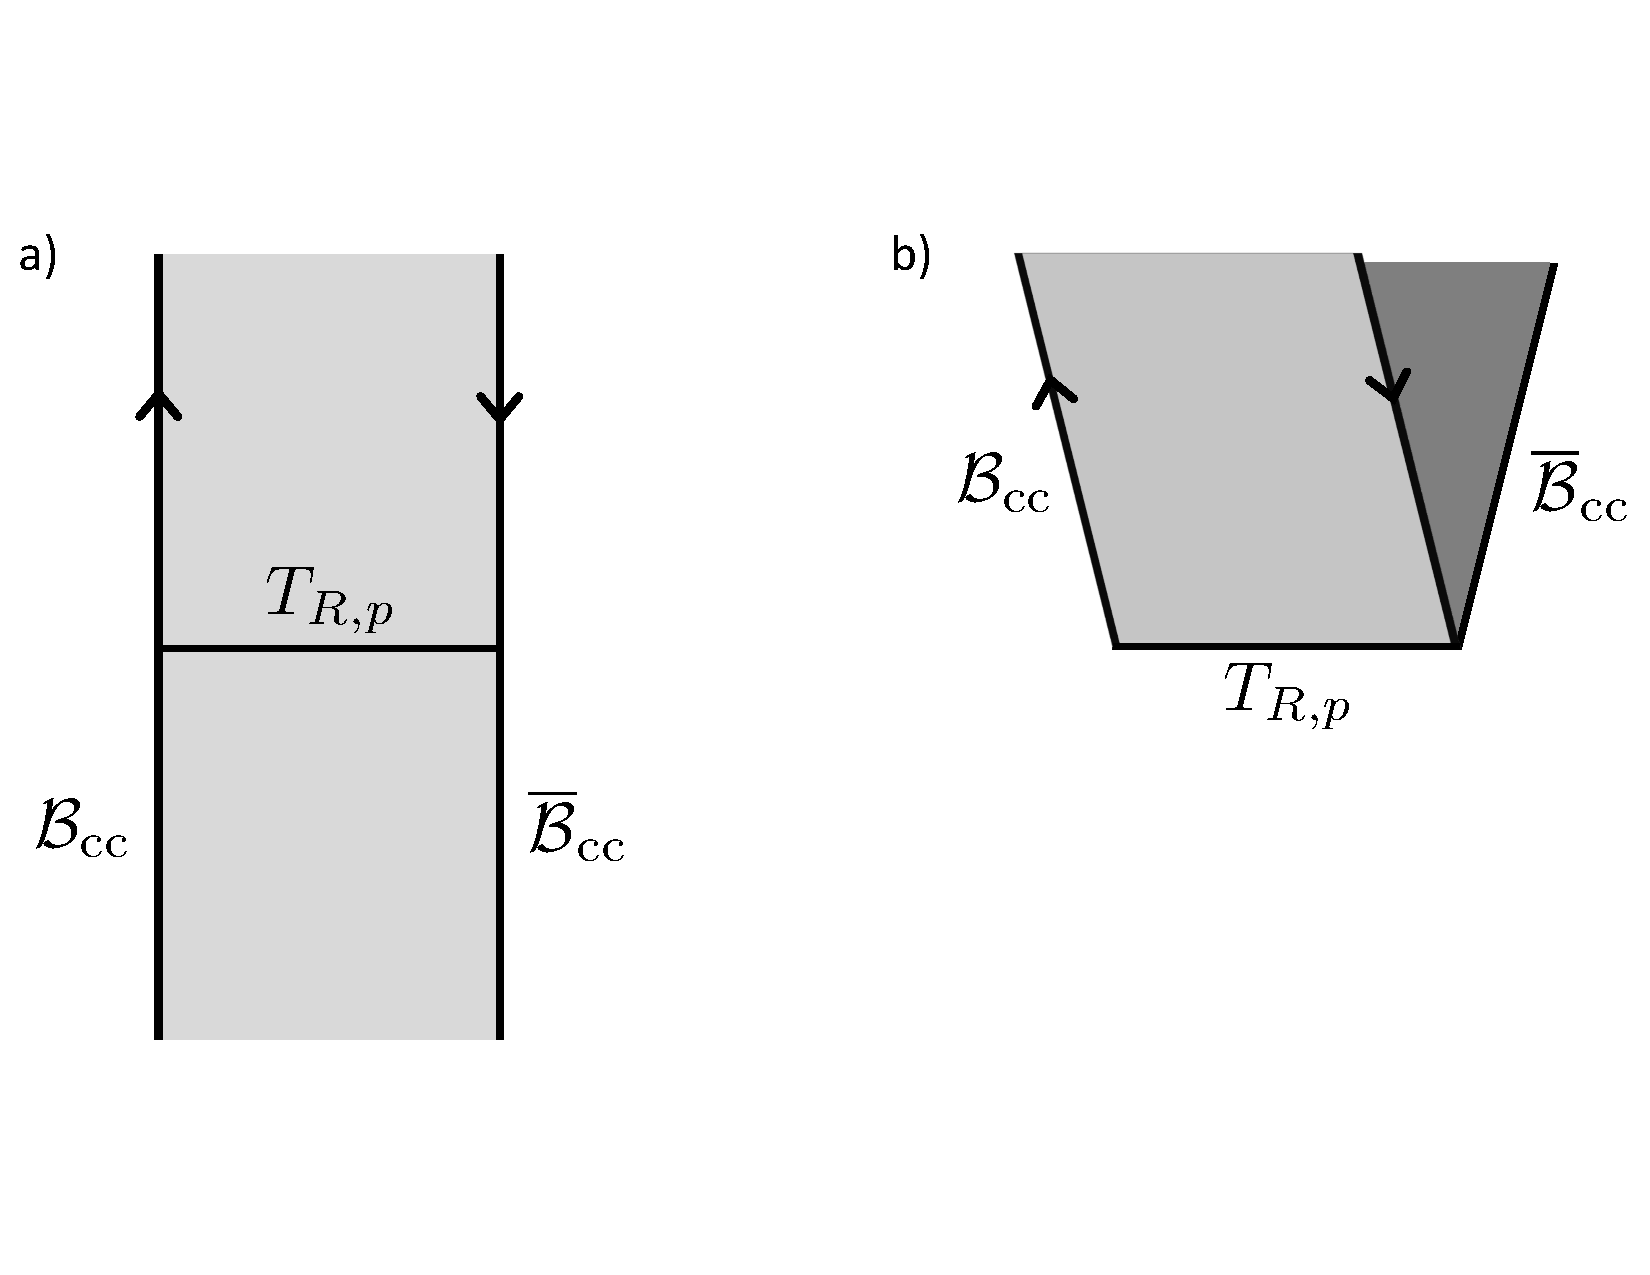
\includegraphics[width=3.6in]{Example7.pdf}
 \end{center}
\caption{\small (a) 把 't Hooft 算符视为从 $\M_H(G,C)$ 的 $A$-模型到自身的界面。(b) 经“折叠”（folding）后，同一个 't Hooft 算符被解释为两张 $\M_H(G,C)$ 之积中的一张膜，它在该乘积中给出一个边界条件；两份辛形式大小相等而符号相反。\label{example7}}
\end{figure} 

\subsubsection{'t Hooft 算符与 Hecke 修正}\label{THO}

一个 't Hooft 算符 $T_{R,p}$（图 \ref{example7}(a)）会使场 $(A,\phi)$ 以及相应的希格斯丛 $(E,\varphi)$ 发生跳跃：'t Hooft 算符紧下方的希格斯丛 $(E,\varphi)$ 一般与紧上方的希格斯丛 $(E',\varphi')$ 不同构。二者之差就是所谓的 Hecke 修正。Hecke 修正的类型由 't Hooft 算符的磁奇异性决定，后者按对偶群 $G^\vee$ 的不可约表示 $R$ 的选取来分类。丛与希格斯丛的 Hecke 修正已在 \cite{KW} 中向物理学家作了说明，\cite{More} 第 4 节给出了更详细的讨论。这里我们只作非常简短的概述。\zy{'t Hooft 算符是磁荷线算符，由对偶群 $G^\vee$ 的不可约表示 $R$ 标记；Wilson 算符是电荷线算符，由所在理论规范群的表示标记。本文的对偶一侧规范群为 $G^\vee$，故 $W_{R,p}$ 也由 $G^\vee$ 的同一表示 $R$ 标记。参见 G. 't Hooft, Nucl. Phys. B138 (1978) 1 及 \cite{KW}。}

全纯 $G_\C$ 丛 $E$ 在点 $p$ 处的 Hecke 修正，是这样一个新丛 $E'$：它带有一个在 $p$ 之外与 $E$ 的同构，但该同构不能延拓到 $p$ 上。$E'$ 的截面 $w$ 就是 $E$ 的截面，只不过允许它在 $p$ 处有指定类型的极点，或受约束使某些分量在 $p$ 处有指定类型的零点，或两者兼有。

例如，设 $E$ 是秩 2 的全纯向量丛，在 $p$ 附近取平凡化，使 $E$ 的截面是一对全纯函数 $\begin{pmatrix}f\cr g\end{pmatrix}$；那么 $E$ 在 $p$ 处的一个 Hecke 修正的例子，是这样一个新丛 $E'$：其截面是一对 $\begin{pmatrix}f\cr g\end{pmatrix}$，其中 $f$ 在 $p$ 处全纯，而 $g$ 允许在 $p$ 处有单极点。这个例子可稍作推广，给出以 $\bCP^1$ 参数化的一族 $E$ 在 $p$ 处的 Hecke 修正。我们只需取一对不全为零的复数 $u,v$，代表 $\bCP^1$ 中一点，并允许 $E'$ 的截面具有与这对数成比例的极点部分：
\be\label{thep} w= \frac{1}{z}\begin{pmatrix}u\cr v\end{pmatrix}+{\mathrm{regular}}, \ee
其中 $z$ 是 $p$ 处的局部参数。

$E$ 与 $E'$ 之间的关系是互反的：与其说我们通过允许某一类型的极点而从 $E$ 得到 $E'$，不如说我们通过要求某一类型的零点而从 $E'$ 得到 $E$。若 't Hooft 算符 $T_{R,p}$ 能把 $E$ 映为 $E'$，则对偶的 't Hooft 算符（与对偶表示相联系）能把 $E'$ 映为 $E$。
 
                                                                    

希格斯丛 $(E,\varphi)$ 的 Hecke 修正实际上对 $\varphi$“什么也没做”。意思是：$(E,\varphi)$ 的 Hecke 修正，就是一个 $E$ 的 Hecke 修正 $E'$，使得 $\varphi:E\to E\otimes K_C$ 作为映射 $E'\to E'\otimes K_C$ 全纯。在秩 2 丛的例子中，希格斯场局部为 $\varphi=\varphi_z\,\d z$，其中 $\varphi_z$ 是 $2\times 2$ 的全纯函数矩阵。要使 $\varphi$ 作为映射 $E'\to E'\otimes K_C$ 全纯，充分必要条件是：若 $w$ 是式 (\ref{thep}) 所刻画的 $E'$ 的截面，则 $\varphi w$ 的极点部分应是 $\begin{pmatrix}u\cr v\end{pmatrix}$ 的倍数；换言之，$\begin{pmatrix}u\cr v\end{pmatrix}$ 必须是矩阵 $\varphi_z(p)$ 的本征向量。一般情形下这一条件并不满足，因此 $E$ 的大多数 Hecke 修正都不能作为 $(E,\varphi)$ 的 Hecke 修正。若 $\varphi_z(p)$ 非幂零，则它有两个不同的本征向量，希格斯丛 $(E,\varphi)$ 在 $p$ 处有两个这种类型的可能 Hecke 修正；若 $\varphi_z(p)$ 幂零但不为零，则它只有一个本征向量，这种类型的可能 Hecke 修正也只有一个；只有当 $\varphi_z(p)=0$ 时，$(E,\varphi)$ 才与 $E$ 本身一样，在 $p$ 处有同一个 $\bCP^1$ 族的这种类型的可能 Hecke 修正。

刚刚描述的这类 Hecke 修正可以从两种不同的角度来看。它们对偶于 $G^\vee=\U(2)$ 的二维表示。该群自对偶，因此上述讨论适用于 $G=\U(2)$ 的规范场论。换一种说法，同一个 Hecke 修正对偶于 $G^\vee=\SU(2)$ 的二维表示。此时对偶群为 $G=\SO(3)$。在这一应用中，由于秩 2 丛 $E$ 与 $E'$ 并不以 $\SO(3)$ 为结构群，前述讨论应以相应的伴丛 $\ad(E)$ 与 $\ad(E')$ 重新表述。

在这个例子中，设 $\delta$ 为 $\varphi(p)$ 作用在 $\begin{pmatrix}u\cr v\end{pmatrix}$ 上的本征值：
\be\label{defdelta} \varphi(p) \begin{pmatrix}u\cr v\end{pmatrix}=\delta \begin{pmatrix}u\cr v\end{pmatrix}.\ee
当 $E$ 与 $E'$ 的选取变化时，$\delta$ 全纯地变化。它定义了这类 Hecke 修正空间上的一个全纯函数。由于 $\varphi(p)$ 的本征值为 $\pm \delta$，我们有
\be\label{delchar} \delta^2=-\det \varphi(p),\ee
其中 $\det\varphi(p)$ 是 Hitchin 哈密顿量的线性组合。$\delta$ 的符号区分与给定希格斯场相容的两种 Hecke 修正。









\subsubsection{Hecke 对应}\label{HC}

't Hooft 算符 $T_{R,p}$ 可以视为 $\M_H(G,C)$ 的 $A$-模型到自身的界面。这不过是同义反复；在图 \ref{example7}(a) 中，我们在 $T_{R,p}$ 的上方与下方都看到 $\M_H(G,C)$ 的 $A$-模型，因此可以把 $T_{R,p}$ 视为这个 $A$-模型的两份副本之间的界面。事实上，由于 $T_{R,p}$ 的超对称性质，这个界面是 $(B,A,A)$ 型的。使用类似于图 \ref{folding} 的折叠技巧会很方便。我们不必把 $T_{R,p}$ 与 $\M_H(G,C)$ 的 $A$-模型中的界面相联系，而可以把它与乘积 $\M_H(G,C)\times \M_H(G,C)$ 的 $A$-模型中的一张 $(B,A,A)$ 型膜或边界条件 $\B_{R,p}$ 相联系（图 \ref{example7}(b)）。这里 $\M_H(G,C)\times \M_H(G,C)$ 的辛结构为 $\omega_K\boxplus (-\omega_K)$，其中一个因子取负号，因为折叠会反转辛结构的符号。

让我们具体看看，对于第 \ref{THO} 节所述的基本例子——$R$ 为 $G^\vee=\SU(2)$ 的二维表示——$\B_{R,p}$ 会是什么样子。它的复维数是多少？若 $C$ 的亏格为 $g$，则 $G_\C$ 丛 $E$ 的选取依赖于 $3g-3$ 个复参数。选取可由 $T_{R,p}$ 作用于 $E$ 而得到的 $E'$，又多出一个复参数。但我们还必须约束希格斯场 $\varphi$，使 $\begin{pmatrix}u\cr v\end{pmatrix}$ 是 $\varphi(p)$ 的本征向量。因此 $\varphi$ 的选取涉及 $3g-4$ 个参数，而不是 $3g-3$ 个。结论是：$\B_{R,p}$ 的支撑 $Z_{R,p}$ 的维数为 $6g-6$，于是 $Z_{R,p}$ 在 $\M_H(G,C)\times \M_H(G,C)$ 中是中维的（middle-dimensional）。由于 $Z_{R,p}$ 是中维的，且是 $(B,A,A)$ 型膜的支撑，它必是复拉格朗日子流形。膜 $\B_{R,p}$ 的秩为 1，因为 $T_{R,p}$ 由 $E$ 产生 $E'$ 所用的 Hecke 变换（若存在）一般是唯一的。简言之，$\B_{R,p}$ 是一张 $(B,A,A)$ 型的秩 1 拉格朗日膜。

我们可以说得更具体些，因为 $\B_{R,p}$ 显然在 $\varphi$ 的标度变换下不变，而这一变换对应于 $\M_H(G,C)\times \M_H(G,C)$ 的 $\C^*$ 对称性。我们可以给出一个简单描述，其意义与用稠密开集 $T^*\M(G,C)$ 近似 $\M_H(G,C)$ 相同。（正如量子化的一般讨论那样，我们预期在 $\lmark^2$ 理论中这一近似是足够的。）$Z_{R,p}$ 与 $\M(G,C)\times \M(G,C)\subset T^*\M(G,C)\times T^*\M(G,C)$ 的交，是参数化配对 $E,E'$ 的簇 $X_{R,p}$，其中 $E'$ 可由 $E$ 经 $p$ 处 $R$ 型 Hecke 变换得到。$Z_{R,p}$ 的 $\C^*$ 不变性意味着它可以被认定为 $X_{R,p}$ 的余法丛\footnote{若子流形 $U\subset M$ 局部由若干坐标 $q_1,\cdots, q_r$ 的零点定义，则它在 $T^*M$ 中的余法丛由令这些坐标以及与它们泊松交换的动量等于零来定义。}。$X_{R,p}$ 在这种情形下称为 Hecke 对应，而 $Z_{R,p}$ 是希格斯丛的 Hecke 对应。
\zy{几何朗兰兹中，Hecke 对应 $X_{R,p}$ 给出 Hecke 函子（沿对应拉回、再推回），Hecke 本征层即其本征对象；希格斯丛的 Hecke 对应 $Z_{R,p}$ 是 $X_{R,p}$ 在 $T^*\M(G,C)\times T^*\M(G,C)$ 中的余法丛。参见 \cite{BD} 与 E. Frenkel, arXiv:hep-th/0512172。}
   
对偶于 $G^\vee=\SU(2)$ 二维表示的这个 't Hooft 算符特例相对简单，因为给定丛 $E$ 在给定点 $p$ 处的可能 Hecke 修正构成一维空间。一般而言，$T_{R,p}$ 能在 $p$ 处对 $E$ 作出的 Hecke 修正，其空间的维数依赖于 $R$；若 $R$ 是 $G^\vee$ 的最高权很大的表示，该维数可任意大。当维数足够大时，每个 $E'\in \M(G,C)$ 都可由 $E$ 经 $T_{R,p}$ 得到，而得到它的方式构成一个正维数的复流形 $\Phi_{E',E,R,p}$。在这种情形下，$Z_{R,p}$ 相当复杂。它有一个希格斯场为零的分支（若 $E'$ 由 $E$ 经一个权非常高的普通 Hecke 修正产生，则不存在非零的 $\varphi:E\to E\otimes K$ 作为映射 $E'\to E'\otimes K$ 全纯），还有希格斯场非零的其他分支（可以选取 $E$ 的权任意高的 Hecke 修正，使得 $\varphi:E'\to E'\otimes K$ 全纯）。$\B_{R,p}$ 的 $\CP$ 丛限制到各分支上并不只是秩 1 的。例如，限制到希格斯场为零的那个分支上，这个 $\CP$ 丛形式地（也就是说，在恰当处理奇点之后）就是 $\Phi_{E',E,R,p}$ 的上同调。
\zy{原文所说的 $\CP$ 丛指膜上的 Chan–Paton 丛，其秩即膜的秩；“并不只是秩 1”指它在某些分支上秩可大于 1。参见 J. Polchinski, \emph{String Theory}, Vol. 1（CUP, 1998）。}
 
\subsubsection{'t Hooft 线算符作为量子态上的算符}\label{lineq}
   
在相当一般的条件下，若辛流形 $M$ 能通过膜量子化得到希尔伯特空间 $\H$，则 $M\times M$ 中的 $A$-膜 $\B$（并在“角”处带有附加数据，详见下文）可解释为 $\H$ 上的量子算符。\cite{GW} 第 4 节对此作了一般讨论。一般说来，很难得到这种算符的显式描述。但这里我们处于一个答案简单的特殊情形。这是因为 $M=\M_H(G,C)$ 实际上就是余切丛 $T^*\M(G,C)$，而所关心的膜支撑在子簇 $X_{R,p}\subset \M(G,C) \times \M(G,C)$ 的余法丛上。
 
作用在 $T^*\M(G,C)$ 的量子化上的相当一般的算符 $\O$，可以用 $\M(G,C)\times \M(G,C)$ 上的半密度 $F(x,y)$ 作为积分核来表示。$\O$ 对态 $\Psi$ 的作用为
\be\label{actst} \O\Psi(x)=\int_{\M(G,C)}\d y \, F(x,y) \Psi(y). \ee
与 't Hooft 算符 $T_{R,p}$ 相联系的量子算符 $\h T_{R,p}$ 应具有何种积分核？式 (\ref{actst}) 中的点 $y$ 与 $x$，在图 \ref{example7}(a) 中对应于线算符 $T_{R,p}$ 紧下方与紧上方的场 $(A,\phi)$。因此它们对应于丛 $E$、$E'$，其中 $E'$ 可由 $E$ 经 $p$ 处 $R$ 型 Hecke 修正得到。于是在经典极限下，$F(x,y)$ 是支撑在 $X_{R,p}$ 上的分布，而 $X_{R,p}$ 参数化这样的配对 $(E,E')$。我们首先考虑的最简单情形，是 $F(x,y)$ 在垂直于 $X_{r,p}$ 的方向上为 delta 函数。更一般地，就其对法向的依赖而言，$F(x,y)$ 可正比于 delta 函数在法向变量中的任意阶导数。\zy{$F$ 与 $\Psi$ 各为半密度，$F(x,y)\Psi(y)$ 是 $y$ 方向的密度，故积分不依赖坐标选取；几何量子化中预量子化态本就是半密度。参见 Bates–Weinstein, \emph{Lectures on the Geometry of Quantization}（AMS, 1997）。}

一般而言，人们会预期对“$F(x,y)$ 支撑在经典对应 $X_{R,p}$ 上”这一论断有量子修正。然而在当前情形没有修正，因为被量子化的辛流形是余切丛 $T^*\M(G,C)$，而对应 $Z_{R,p}$ 是 $T^*\M(G,C)\times T^*\M(G,C)$ 中的余法丛。余切丛与余法丛的标度不变性意味着核 $F(x,y)$ 不能依赖于 $\hbar$，并可在半经典极限下计算。

我们应补充说明，为什么在这里依据标度对称性作论证是正当的。膜量子化一如既往，是在某个适当的复化中研究 $T^*\M(G,C)$。类似地，在膜量子化中研究 $Z_{R,p}$，需要把它复化到 $T^*\M(G,C)\times T^*\M(G,C)$ 的某个复化之中。膜量子化中的标度论证实际上涉及复化的标度变换。这种论证在当前情形有效，是因为 $T^*\M(G,C)$ 作为余切丛的结构、以及 $Z_{R,p}$ 作为余法丛的结构，确实延拓为它们复化上的同类型全纯结构。

我们还应当澄清“半经典极限”的含义。波函数是半密度而非函数、相应地 $F(x,y)$ 是 $\M(G,C) \times \M(G,C)$ 上的半密度，这一论断本身已包含单圈修正。说 $F(x,y)$ 可以半经典地计算，意思是除此之外没有别的量子修正。

根据 Etingof、Frenkel 与 Kazhdan \cite{EFK2}，对偶于 $\SU(2)$ 二维表示的 Hecke 算符由一个积分核定义，该核可分解为全纯因子与反全纯因子之积。这种全纯因子化在 $A$-模型中是可预期的。全纯因子 $f$ 将来自图 \ref{example7}(a) 中 $T_{R,p}$ 的左端点，等价地来自图 \ref{example7}(b) 的左下角；反全纯因子 $\t f$ 将来自右端点或右下角。
我们把 't Hooft 算符视为 $\M_H(G,C)\times \M_H(G,C)$ 中一张 $(B,A,A)$ 型的秩 1 膜，其 $\CP$ 丛平凡。一般而言，这种支撑在拉格朗日子流形 $L$ 上的膜与典范余迷向 $A$-膜之间的角空间为 $H^0(L,K_L^{1/2})$。't Hooft 算符对应于支撑为 Hecke 对应 $Z_{R,p}$ 的膜。因此在这一情形，全纯的角是全纯截面 $f\in H^0(Z_{R,p},K^{1/2}_{Z_{R,p}})$。类似地，反全纯的角是元素 $\t f\in H^0(\bar Z_{R,p},\bar K^{1/2}_{\bar Z_{R,p}})$，其中 $\bar Z_{R,p}$ 是取相反复结构的 $Z_{R,p}$。
 
 
  
$f$ 与 $\t f$ 的乘积 $\mu = f \t f$ 将是 $Z_{R,p}$ 上的半密度。我们将说明，这些数据恰好是定义分布核 $F(x,y)$ 所需。若 $f$ 与 $\tilde f$ 是自 $X_{R,p}$ 拉回的，我们将得到 delta 函数核。若它们对 $Z_{R,p} \to X_{R,p}$ 的纤维有多项式依赖，我们将得到 delta 函数各阶导数的线性组合。

为了描述 delta 函数分布，我们选取一些局部坐标。用 $\M(G,C)$ 上的坐标 $\vec x=x_1,\cdots, x_{3g-3}$ 参数化 Hecke 变换的输入。我们将用 $|\d \vec x|$ 表示半密度 $(\d x_1 \cdots \d x_{3g-3} \d \bar x_1 \cdots \d \bar x_{3g-3})^{1/2}$，对随后引入的其他变量也作同样的理解。给定 $\vec x$ 后，Hecke 变换的输出跑遍一个 $\bCP^1$ 的副本，我们称之为 $\bCP^1_x$，并用复变量 $z$ 参数化它。$\bCP^1_x $ 在 $\M(G,C)$ 中的复余维为 $3g-4$。$\bCP^1_x$ 可局部由条件 $\vec n=0$ 定义，其中 $\vec n=(n_1,\cdots, n_{3g-4})$ 是 $\M(G,C)$ 中 $\bCP^1_x$ 的法丛 $N$ 上的局部全纯坐标。于是核可写为
\be\label{nuff} 
F(x,y)= b(z,\bar z,x, \bar x)|\d\vec x ||\d z \d \vec n |\delta(\vec n,\vec{\bar n})
\ee
其中 $\d \vec n=\d n_1 \d n_2\cdots \d n_{g-4}$，delta 函数由 $\int \d \vec n \d \vec{ \bar n}\delta(\vec n,\vec{\bar n})=1$ 定义。由后一关系可知，在法丛上作坐标变换时，delta 函数按 $(\d \vec n \d \vec{\bar n})^{-1}$ 变换；这意味着可能的核与下列对象一一对应：
\be\label{luff} \mu = b(z,\bar z,x, \bar x)|\d\vec x| |\d z(\d \vec n)^{-1}|. \ee
希格斯丛的 Hecke 对应 $Z_{R,p}$ 局部由上文引入的坐标 $\vec x$ 与 $z$（它们参数化丛的 Hecke 对应 $X_{R,p}$）以及参数化希格斯场选取的附加变量 $\vec m$ 来参数化。由于 $Z_{R,p}$ 是 $X_{R,p}$ 的余法丛，变量 $\vec m$ 与式 (\ref{nuff}) 中出现的法丛坐标 $\vec n$ 对偶。因此我们可以把 $(\d\vec n)^{-1}$ 换成 $\d \vec m$，而可能的 delta 函数核与 $Z_{R,p}$ 上的半密度一一对应：
\be\label{luff1} \mu = b(z,\bar z,x, \bar x)|\d\vec x \d z\d \vec m|^2. \ee
其中 $b$ 与 $\vec m$ 无关。

这一讨论可直接推广到 delta 函数法向导数的线性组合。一个涉及 delta 函数法向导数的核
\be\label{nuff2} 
F(x,y)= b(x, \bar x,z,\bar z, \partial_{\vec n}, \partial_{\vec {\bar n}}) |\d\vec x | |\d z \d \vec n |\delta(\vec n,\vec{\bar n})
\ee
对应于半密度
\be\label{luff2} \mu = b(x, \bar x, z,\bar z,\vec m, \vec {\bar m})|\d\vec x \d z\d \vec m|. \ee
这些半密度定义在 $Z_{R,p}$ 上，且 $b$ 对 $\vec m$ 有多项式依赖。

全纯因子化的核将取 $\mu = f \t f$ 的形式，其中 $f$ 与 $\t f$ 分别是全纯与反全纯的。现在可以看出 $f$ 必须是何种全纯对象。$f$ 必须是 Hecke 对应 $Z_{R,p}$ 上全纯意义下的半密度：$f=v(\vec x, z,\vec m) (\d \vec x\d z\d\vec m)^{1/2}$。用更标准的语言，$f$ 必须是 $H^0(Z_{R,p}, K^{1/2}_{Z_{R,p}})$ 中的元素。如前所述，这正是 $A$-模型中对 $T_{R,p}$ 左端点的答案所应取的形式。类似地，$\t f$ 是 $Z_{R,p}$ 的反典范丛的反全纯截面，这同样符合 $A$-模型的预期。


当且仅当 $Z_{R,p}$ 是 Calabi–Yau 流形时，$K_{Z_{R,p}}^{1/2}$ 存在一个处处非零的特定全纯截面 $\lambda_0$。若这样的 $\lambda_0$ 存在，则定义任何其他全纯角的数据为 $f= g \lambda_0$，其中 $g$ 是 $Z_{R,p}$ 上的全纯函数。特别地，这样的函数 $g$（只具有多项式增长）是 Hitchin 哈密顿量 $H_{\P,\alpha}$ 与式 (\ref{defdelta}) 所定义的全纯函数 $\delta$ 的多项式，但要模去关系 $\delta^2 = -\det \varphi(p)$——该关系把 $\delta^2$ 表示成 $H_{\P,\alpha}$ 的线性组合。非常数多项式 $g(H_{\P,\alpha},\delta)$ 有非平凡的零点，因此 $g\lambda_0$ 处处非零仅当 $g$ 为常数；这表明 $\lambda_0$（若存在）在相差常数倍的意义下唯一。\footnote{更一般地，若 $Z$ 是满足 $b_1(Z)=0$ 的复流形，则 $Z$ 上处处非零、且没有指数增长的全纯函数 $g$ 必为常数。事实上，由 $b_1(Z)=0$，闭 1-形式 $\d g/g$ 恰当，即 $\d g/g=\d w$ 对某个 $w$ 成立，于是 $g=C e^w$（$C$ 为非零常数）；除非 $g$ 为常数，否则 $g$ 有指数增长。$G_\C$-丛的 Hecke 对应满足 $b_1(X_{R,p})=0$。$G_\C$ 希格斯丛的 Hecke 对应是 $X_{R,p}$ 的余法丛，因此 $b_1(Z_{R,p})=0$。}\zy{译者按（无外部依据）：$K^{1/2}_Z$ 有处处非零全纯截面，当且仅当 $K_Z$ 平凡——若 $s$ 是这样的截面，则 $s^2$ 即 $K_Z$ 的处处非零全纯截面，反之亦然。}
形如 $g \lambda_0$ 的角（其中 $g$ 是 Hitchin 哈密顿量与 $\delta$ 的多项式），恰好与 Wilson 线的角相匹配——后者由 $s$、$Ds$ 以及对偶于 Hitchin 哈密顿量的可观测量的多项式构成。


这样的 $\lambda_0$ 确实存在，这归功于 Beilinson 与 Drinfeld 的一个结果 \cite{BD}，该结果在 Etingof、Frenkel 与 Kazhdan 的工作 \cite{EFK2} 中很重要。$\lambda_0$ 的性质映照了第 \ref{wilop} 节中最简单的 Wilson 线角 $s$ 的性质。特别地，根据 Beilinson 与 Drinfeld 的结果，$\lambda_0$ 与 $s$ 一样，作为 $K_p^{-1/2}$ 的截面随 $p$ 变化。当然，这样的 $s$ 的镜像的存在性可由电–磁对偶预期。
 
\cite{EFK2} 中使用了一个稍有不同的表述。为说明这一点，让我们回到式 (\ref{luff})：由此可以看出，若 $\mu$ 能全纯因子化，则其全纯因子是全纯形式 $k = w(\vec x,z) (\d \vec x    \d z)^{1/2}  (\d \vec n)^{-1/2}$。我们可以把 $\d z^{1/2} (\d\vec n)^{-1/2}$ 换成 $\d z (\d \vec y)^{-1/2}$，其中 $\vec y=(z,\vec n)$ 参数化 Hecke 变换的输出。换言之，全纯因子化的核将来自一个全纯对象\footnote{由于 $\vec y$ 由 $\vec x$ 与 $z$ 决定，且反过来 $\vec x$ 由 $\vec y$ 与 $z$ 决定，我们同样可以写 $w(\vec y,z)$ 而不写 $w(\vec x,z)$。}
 \be\label{conf} k=w(\vec x,z) (\d \vec x)^{1/2} (\d\vec y)^{-1/2}\d z. \ee 
若把 $k$ 乘以它的复共轭，我们得到
 \be\label{onf}|k|^2= |w(\vec x,z)|^2 |\d\vec x| |\d z\d\bar z| |\d\vec y|^{-1}.\ee
这直接导致 \cite{EFK2} 中所用的定义。量 $|k|^2$ 可视为从 $\vec y$ 中的半密度到 $\vec x$ 中的半密度的映射，取值于可在 $\bCP^1_x$ 上积分的微分形式 $|\d z \d\bar z|$。该积分给出点 $p\in C$ 处的 Hecke 算符：
 \be\label{tonf} H_p=\int_{\bCP^1_x} |k|^2. \ee
  
 
 
在第 \ref{sec:chiral} 节中，我们将通过二维手征代数来解释其中一些陈述。特别地，第 \ref{fft} 节中关于伴随值手征费米子的讨论，是 Beilinson 与 Drinfeld 原始分析的物理学解释。手征代数方法在 $C$ 上是局部的，并有可能延拓到如下情形：联系两个给定丛的 Hecke 修正空间具有正维数。


\subsubsection{仿射 Grassmann 流形}\label{affgr}


至此我们考虑的都是 Hecke 修正的最简单例子。但要把理论进一步发展，人们需要更系统的途径。

作为动机，我们首先考虑秩 $n$ 的全纯向量丛。设 $z$ 是在点 $p\in C$ 处为零的局部全纯参数，$U$ 是 $p$ 的小邻域。$C$ 有一个由两个开集组成的开覆盖，即 $U$ 与 $C'=C\backslash p$（从 $C$ 中挖去 $p$）。在点 $p$ 的小邻域 $U$ 中取 $E$ 的平凡化，并把 $E$ 限制到 $C'$。设 $E_0\to U$ 是秩 $n$ 的平凡向量丛。于是我们得到 $C$ 的一个开覆盖，由开集 $C'$ 与 $U$ 组成，其上分别有向量丛 $E\to C'$ 与 $E_0\to U$。因此可以通过在 $U'=C'\cap U$ 上把 $E$ 与 $E_0$ 用一个规范变换粘合起来，定义新的向量丛 $E'\to C$。例如，我们可以用从 $E_0$ 到 $E$ 的对角规范变换
  \be\label{gtr} g(z) =\begin{pmatrix} z^{d_1} &&&\cr
                                                                      & z^{d_2} &&\cr
                                                                       &&\ddots & \cr
                                                                          &&& z^{d_n}\end{pmatrix},\ee 其中 $d_1,\cdots, d_n$ 为整数。
对于 $G=\U(n)$，适当选取 $d_i$，这就给出一个 $G_\C$-丛的 Hecke 修正的例子，它对偶于 $G=\U(n)$ 的任意不可约有限维表示。
对于 $G=\SU(n)$，只需再要求 $\sum_i d_i=0$，使 $g(z)$ 取值于 $\SL(n,\C)$；对于 $G=\PSU(n)$，则考虑 $d_i$ 取值于 $\frac{1}{n}\Z$，且 $d_i-d_j\in \Z$（这等价于说：若把 $g(z)$ 写在 $\PSU(n)$ 的表示中，则只出现 $z$ 的整数幂）。把所有 $d_i$ 作常数平移 $d_i\to d_i+c$（其中 $c\in \Z$，对 $G=\PSU(n)$ 则 $c\in \frac{1}{n}\Z$）不影响 Hecke 修正的空间，因为这可以通过 $E'\to E'\otimes \O(p)^c$ 补偿。


对任意 $G$，都可作类似构造：把其元素为 $z$ 的各次幂的对角矩阵换成同态 $g(z)= z^\m :\C^*\to T_\C$，其中 $\C^*$ 是挖去原点的 $z$ 平面，$T_\C$ 是 $G_\C$ 的复极大环面，而 $\m$ 推广了上一段中的整数 $d$ 元组 $(d_1,\cdots, d_n)$，它是对偶群 $G$ 的整权，在物理上对应于 't Hooft 算符的磁荷。


至此所描述的是对偶于 $G$ 的任意有限维表示 $R$ 的 Hecke 变换的标准例子；$R$ 由整数 $d_i$ 或 $\m$ 的选取所编码。
这一构造依赖于最初在 $U$ 上对 $E$ 的平凡化的选取。通过改变平凡化的选取，可以得到同一类型 Hecke 修正的整个空间。一旦选定一个参考平凡化，$E$ 在集合 $U$ 上的任何其他平凡化都可由参考平凡化经
某个在 $U$ 上全纯的规范变换 $g'(z)$ 作用得到。与此替代平凡化相应的标准 Hecke 修正，在参考平凡化下由修改后的奇异规范变换 $g'(z) z^\m$ 描述。
 
两个奇异规范变换给出同一个 $E'$，当且仅当它们可以通过从右复合一个定义在 $U$ 上的规范变换 $g''(z)$ 相互联系。于是，$E$ 的两个平凡化给出同一个标准 Hecke 修正，当且仅当相应的规范变换 $g_1'(z)$ 与 $g_2'(z)$ 满足
\begin{equation}
g_1'(z)z^\m = g_2'(z)z^\m g''(z)
\end{equation}
对某个 $g''(z)$ 成立。

这些关系可以借助{\it 仿射 Grassmann 流形} $\Gr_{G_\C}$ 来形式化。习惯上把定义在 $U'$ 上的 $G_\C$ 值规范变换构成的（无穷维）空间记作 $G_\C[{\cal K}]$，并把其中可全纯延拓到 $U$ 的子空间记作 $G_\C[{\cal O}]\subset G_\C[{\cal K}]$。仿射 Grassmann 流形
\begin{equation}
\Gr_{G_\C} \equiv G_\C[{\cal K}]/G_\C[{\cal O}]
\end{equation}
参数化的是奇异规范变换的等价类。我们定义 $\Gr^\m_{G_\C}$ 为 $\Gr_{G_\C}$ 中由粘合函数 $z^\m$ 给出的标准 Hecke 修正所在的轨道：
\begin{equation}
\Gr^\m_{G_\C} \equiv \left[G_\C[{\cal O}] z^\m \right].
\end{equation}
$\Gr^\m_{G_\C}$ 中的每一点都在某个这样的轨道上（对某个 $\m$）。
\begin{yizhu}[译者按：仿射 Grassmann 流形与 Hecke 修正]
原文用 $\Gr_{G_\C}=G_\C[{\cal K}]/G_\C[{\cal O}]$ 来表述 Hecke 修正，其中 ${\cal K}=\C((z))$、${\cal O}=\C[[z]]$ 为形式洛朗级数环与形式幂级数环。直观上，$\Gr_{G_\C}$ 的参数是“在穿孔邻域 $U'$ 上平凡、在 $p$ 处允许有极点”的 $G_\C$-丛粘合数据；$\Gr^\m_{G_\C}$ 则是粘合函数 $z^\m$ 所在的轨道。对 $G=\U(n)$，轨道由 $n$ 元组 $(d_1,\cdots,d_n)$ 模去整体平移刻画，同时平移所有 $d_i$ 相当于把丛张量以 $\O(p)$ 的某个幂，不改变 Hecke 修正的空间。原文后文 $|d_i-d_j|\leq 1$ 的条件选出的正是极小（minuscule）轨道，故不发生单极子冒泡。介绍见 X. Zhu, “An introduction to affine Grassmannians and the geometric Satake equivalence,” arXiv:1603.05593；用法见 \cite{BD}。
\end{yizhu}


对 $G$ 与 $\m$ 的一般选取，会遇到“单极子冒泡”（monopole bubbling）现象：'t Hooft 算符或 Hecke 算符的磁荷可能发生向下跳跃（这一现象由 \cite{Kron,Pauly} 引入；简短介绍见 \cite{KW} 第 10.2 节）。本质上，轨道 $\Gr^\m_{G_\C}$ 在仿射 Grassmann 流形中不是闭的，其（可能奇异的）闭包包含磁荷更小的其他轨道 $\Gr^{\m'}_{G_\C}$。这会使分析大为复杂化。

对 $G=\U(n)$ 或与之相关的群 $\SU(n)$、$\mathrm{PSU}(n)$，避免单极子冒泡的条件是对所有 $i,j$ 有 $|d_i-d_j|\leq 1$。在把所有 $d_i$ 作常数平移（如式 (\ref{gtr}) 的讨论所述，这不影响 Hecke 修正的空间）之后，为避开单极子冒泡，可以假定 $k$ 个 $d_i$ 为 $-1$，其余为 $0$。
具体地说，这对应于如下类型的 Hecke 修正。设 $E\to C$ 是秩 $n$ 的全纯向量丛，$p\in C$；选取一个 $k$ 维子空间 $V\subset E_p$，定义新向量丛 $E'\to C$，其截面是 $E$ 的截面中允许在 $p$ 处有单极点、且留数落在 $V$ 中的那些。这类 Hecke 修正的空间由 $V$ 的选取参数化，也就是由 $E_p$ 的 $k$ 维子空间构成的 Grassmann 流形参数化。这样的 Hecke 修正对偶于 $G=\U(n)$ 或 $\SU(n)$ 的基本表示的 $k$ 次反对称幂。
在这一情形，$\varphi$ 在 $w$ 的极点部分上表现为 $k \times k$ 矩阵。$\varphi$ 的 $k \times k$ 限制的特征多项式取一般形式 $u(x) = x^k + \delta_1 x^{k-1} + \cdots \delta_k$，其中 $\delta_1,\cdots, \delta_k$ 是某些全纯函数。这些函数与 Hitchin 哈密顿量 $\H_{\P,\alpha}(\varphi)$ 满足多项式关系，这些关系编码了“$u(x)$ 整除 $\varphi$ 的特征多项式”这一约束。




% \subsubsection{Corner data for 't Hooft Line Operators}
%In the brane quantization setup we need to identify good choices of corner morphisms $\alpha$ which can represent supersymmetric 
%endpoints of 't Hooft lines on the deformed Neumann boundary conditions. In a classical approximation, such endpoints are 
%labelled by holomorphic functions on the $Z_{R,p}$ correspondence. In order to compare 't Hooft and Wilson line observables, we 
%need to be able to compare the respective endpoints. 
%
%In the case of $\SO(3)$ and the minimal charge 't Hooft loop, we have identified above a holomorphic observable $\delta$. This represents a holomorphic function on $Z_{2,p}$ which does not descend from a holomorphic function on $\M(G,C)\times \M(G,C)$. Instead, it satisfies the relation $\delta^2 = \frac12 \Tr \varphi^2(p)$. We thus have two candidate ``classical corners'', labelled by holomorphic functions $1$ and $\delta$. 
%
%On the $S$-dual side, we also have two corners: the canonical holomorphic section $s$ and its first derivative $Ds$. We also have a relation $D^2s = t s$ which closely resembles a quantization of the $\delta^2 = \frac12 \Tr \varphi^2(p)$ relation. The resemblance becomes particularly close when we observe that the holomorphic function $\delta$ is actually the Hamiltonian for the infinitesimal deformation $Z_{2,p} \to Z_{2, p + d p}$, 
%i.e. if we let $p$ vary as we compute the difference of complex symplectic forms on $\M_H(G,C)\times \M_H(G,C)$ we obtain $d\delta dp$. 
%Correspondingly, multiplication of a holomorphic function by $\delta$ is the classical approximation to a $D$ derivative acting on a corner. 
%Similar considerations apply to the case of minimal charge 't Hooft loops for $\mathrm{PSU}(n)$. 
%
%Remarkably, the quantum numbers of the classical corners $1$ and $\delta$ do not match the quantum numbers of the Wilson line corners: 
%$s$ is a section of $K_C^{-\frac12}$ while $1$ is not. We will now explain now how such mismatch can be corrected at the semiclassical level. 
%
%\subsubsection{??}
%
%Consider the case of $G=\SO(3)$ and minimal Hecke modification. After selecting a local description in the neighbourhood of $p$, the 
%space of Hecke modifications is $\CP^1$ and we we should thus write 
%\be\label{actst2} \O_{2} \Psi(x)=\int_{\CP^1}|\d z| \left|\frac{\d(H_z \circ x)}{\d y} \right| \, F(z,x) \Psi(H_z \circ x) . \ee
%where $x$ represents $E$, $H_z \circ x$ represents $E'$ and $z$ is a point on $\CP^1$. For later convenience, we inserted an explicit 
%Jacobian factor, comparing the bundle of half-densities in a neighbourhood of $E$ and $E'$.
%
%Next, we impose the constraint that the 't Hooft operator is local on $C$. In particular, the weight give to a specific Hecke modification cannot depend on the structure of the bundle away from $p$, nor on the specific direction of the Hecke modification, as the direction can be changed by a different choice of local trivialization of the bundle $E$. We thus propose 
%\be\label{actst3} \O_{2} \Psi(x)=\int_{\CP^1}|\d z| \left|\frac{\d(H_z \circ x)}{\d y} \right| \, \Psi(H_z \circ x) . \ee
%This proposal actually makes sense because of a rather non-trivial fact: the Jacobian factor transforms as a density on the space of Hecke modifications. 
%
%The Jacobian factor has another remarkable property: it depends on $p$ as a section of $|K_C|^{-1}$. As a consequence, 
%the operator $\O_2$ has precisely the same quantum numbers as the minimal Wilson operator on the dual side, $s \wedge \bar s$. 
%
%As for other important properties of the space of bundles, these properties of the Jacobian are easiest to derive in the model given by the space of 2d connections modulo complexified gauge transformations, where chiral algebra methods become available. We will do so in a dedicated section of the paper. The same methods also allow one to verify the differential equation $D_p^2 O_2 = D_{\P} O_2$ expected from $S$-duality: the 
%'t Hooft line endpoints satisfy an oper differential equation with a classical stress tensor given by the quantum Hitchin Hamiltonians. 
%
%Notice that the other non-trivial corner, obtained as $D_p O_2$, gives an integral-differential operator. This is the sort of operator which one may associate to the quantization of a conormal correspondence with non-trivial corners. 
%
%Important elements of this analysis apply to general gauge group $G$ and magnetic charge $\lambda$. We would seek an integral operators defined tentatively as an integral over some space ${\cal H}_\lambda$ of Hecke modifications:
%\be\label{actst4} \O_{\lambda} \Psi(x)=\int_{{\cal H}_\lambda}|\d z| \left|\frac{\d(H_z \circ x)}{\d y} \right| \,  F(z,x)  \Psi(H_z \circ x) . \ee
%The local change of trivializations act on ${\cal H}_\lambda$. Indeed, a natural choice of ${\cal H}_\lambda$ is the closure of the orbit of 
%the $z^\lambda$ modification under the action of local changes of trivialization. It is thus natural to set $F(z,x)=1$ and hope that 
%the Jacobian will give a reasonably behaved density on the space ${\cal H}_\lambda$. 
%
%Such operators are the natural candidate dual to the leading Wilson line operators $(\bar s_{\bar R_\lambda}, s_{R_\lambda})$
%in the representation $R_\lambda$ labelled by $\lambda$. A very non-trivial check of this proposal would be a comparison of 
%the differential equations satisfied by the two sides. Again, this is ultimately a chiral algebra calculation. 
%
%One can also seek more general integral-differential operators which integrate over ${\cal H}_\lambda$ some combination of derivatives 
%of $\Psi$, possibly generating operators which are $S$-dual to more general $(\bar s_{\bar R_\lambda,\bar n}, s_{R_\lambda,n})$.
%
%


    
 
